
%(BEGIN_QUESTION)
% Copyright 2006, Tony R. Kuphaldt, released under the Creative Commons Attribution License (v 1.0)
% This means you may do almost anything with this work of mine, so long as you give me proper credit

Bestem trykket ved hver port på DP-transmitteren under en instrumentteknikers trinnvise ventil-isolasjonsprosedyre.  Anta at prosessmediet som transmitteren måler er en gass og ikke en væske:

$$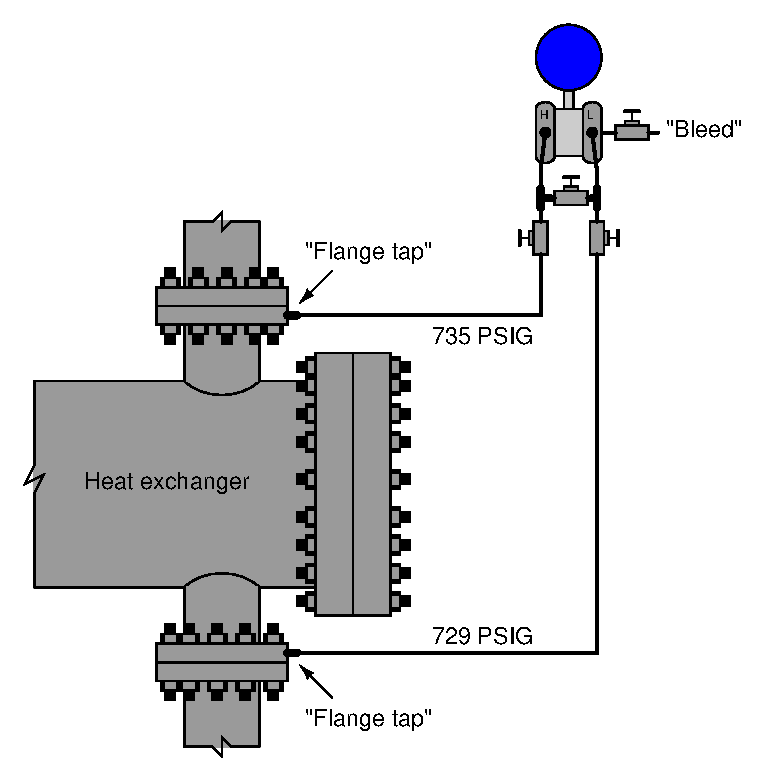
\includegraphics[width=15.5cm]{i00026x01.eps}$$

% No blank lines allowed between lines of an \halign structure!
% I use comments (%) instead, so that TeX doesn't choke.

$$\vbox{\offinterlineskip
\halign{\strut
\vrule \quad\hfil # \ \hfil & 
\vrule \quad\hfil # \ \hfil & 
\vrule \quad\hfil # \ \hfil \vrule \cr
\noalign{\hrule}
%
% First row
Step & High-side pressure & Low-side pressure \cr
%
\noalign{\hrule}
%
% Another row
1: Transmitter in service &  &  \cr
%
\noalign{\hrule}
%
% Another row
2: Close high-side block valve &  &  \cr
%
\noalign{\hrule}
%
% Another row
3: Close low-side block valve &  &  \cr
%
\noalign{\hrule}
%
% Another row
4: Open equalizing valve &  &  \cr
%
\noalign{\hrule}
%
% Another row
5: Open bleed valve &  &  \cr
%
\noalign{\hrule}
} % End of \halign 
}$$ % End of \vbox

Basert på de viste prosesstrykkene, identifiser retningen på prosessgassen gjennom denne varmeveksleren.

\vskip 10pt

Identifiser også hva teknikeren må fortelle prosessoperatøren(e) før han isolerer transmitteren fra denne prosessen.

\vfil

\underbar{file i00026}
\eject
%(END_QUESTION)





%(BEGIN_ANSWER)

Dette er et vurdert spørsmål -- ingen svar eller hint gis!

%(END_ANSWER)





%(BEGIN_NOTES)

Når utjevningsventilen åpnes {\it etter} at begge blokkventilene er stengt, vil trykkene mellom de to sidene av transmitterens målekapsel ha en tendens til å utjevnes.  Dermed vil 735 PSI fanget på høy side og 729 PSI fanget på lav side bli omtrent 732 PSI på begge sider etter at utjevningsventilen er åpnet:

% No blank lines allowed between lines of an \halign structure!
% I use comments (%) instead, so that TeX doesn't choke.

$$\vbox{\offinterlineskip
\halign{\strut
\vrule \quad\hfil # \ \hfil & 
\vrule \quad\hfil # \ \hfil & 
\vrule \quad\hfil # \ \hfil \vrule \cr
\noalign{\hrule}
%
% First row
Step & High-side pressure & Low-side pressure \cr
%
\noalign{\hrule}
%
% Another row
1: Transmitter in service & 735 PSI & 729 PSI \cr
%
\noalign{\hrule}
%
% Another row
2: Close high-side block valve & 735 PSI & 729 PSI \cr
%
\noalign{\hrule}
%
% Another row
3: Close low-side block valve & 735 PSI & 729 PSI \cr
%
\noalign{\hrule}
%
% Another row
4: Open equalizing valve & 732 PSI & 732 PSI \cr
%
\noalign{\hrule}
%
% Another row
5: Open bleed valve & 0 PSI & 0 PSI \cr
%
\noalign{\hrule}
} % End of \halign 
}$$ % End of \vbox

En måte å se for seg utjevningen av trykk i trinn \#4 er å forestille seg hva som skjer hvis to bildekk med ulikt lufttrykk kobles sammen med et rør.  Siden Pascals prinsipp sier at et trykksatt fluid i et lukket volum vil forsøke å fordele trykket likt, vil luftmolekylene i dekket med høyere trykk strømme gjennom røret og inn i dekket med lavere trykk for å utjevne trykket.  Dermed tappes det høytrykkede dekket for noe luft, mens det lavtrykkede får litt luft.  Til slutt vil trykket i begge dekk være likt, og trykkverdien vil ligge et sted mellom de to opprinnelige trykkene.

\vskip 10pt

Strømningen av prosessgass gjennom denne varmeveksleren er {\it inn} på toppen og {\it ut} i bunnen.  Du kan tenke på dette i form av spenningsfall over en motstand i en DC-krets: potensialet er alltid størst (mest positivt) der strømmen (konvensjonell strømretning) går inn.

\vskip 10pt

Før transmitteren isoleres fra prosessen, må teknikeren varsle operatøren om at transmitteren tas ut av drift.  I forberedelse til dette må enhver regulator som er avhengig av denne transmitteren for prosessverdien (PV) settes i manuell modus, og operatørene må se på et annet trykk-indikerende instrument for å kunne styre trykkfallet manuelt mens transmitteren er ute av drift.  Eventuelle prosessalarmer som utløses av transmittersignalet må også deaktiveres slik at det ikke genereres falske alarmer når teknikeren tar transmitteren ut av drift.

%INDEX% Measurement, pressure: 3-valve manifold operation
%INDEX% Process: heat exchanger pressure drop measurement (generic)

%(END_NOTES)
